\chapter{Implementation and results}
\label{kap:kap4}

In this chapter, we describe the implementation of ideas proposed in the previous
chapter and practical results we obtained when measuring experimentally their performance.
This chapter is split into two main parts according to the two main topics discussed
in previous chapter namely our new encoding and decoding method and hybrid encoding.
In both of these sections, we first describe the important parts and decisions in our
implementation. Subsequently, we describe how we benchmarked our implementation and present
the results we obtained.

The source code to all benchmarks can be found in electronic attachment to this work
and also on \texttt{Github}. More about where to find individual parts of code and how
to reproduce our results can be found in
appendix A. All the results presented in this chapter were obtained on a machine with
8-core AMD~Ryzen~7~2700X with 16~MB of cache, running at 3.7~GHz with 16~GB of RAM.
The running operating system was Ubuntu~20.04.3~LTS. We used both \texttt{GCC} version
9.4.0 and \texttt{Clang} version 10.0.0 compilers with the optimizations level most of
the time set to \texttt{O3}. Although there are no special hardware requirements, to
obtain the best possible results, our implementation requires a processor with support
for \texttt{SSE2} instruction set.

\section{New decoding method}

\subsection{Implementation}

\paragraph{SDSL library}

We decided to make our solution a part of the \texttt{SDSL} library~\citep{gog2014theory}. This
is one of the most matured and versatile libraries implementing succinct data structures.
With almost 2\,000 commits from more than 30 contributors, \texttt{SDSL} is a heavily tested library
offering various implementations of succinct structures such as wavelet tree, FM-index,
bit vector, suffix array and many more. It allows easy use of different building blocks
to implement more complex structures, i.e. using different bit vector implementations inside
of the wavelet tree. On top of this, thorough tests and benchmarks were implemented alongside
the main functionality. The RRR implementation is provided by templated class \texttt{rrr\_vector}
that generally uses the on the fly-decoding enabling us to use block sizes from 3 up to 256. To support
these long block sizes, \texttt{SDSL} implements 128-bit and 256-bit integers. On top of this, \texttt{SDSL}
provides template specialization for block size 15 that uses the table decoding method. To support $\access$,
\texttt{rrr\_vector} supports single bit access operator \texttt{[]} as well as \texttt{get\_int} method.
To facilitate $\access$ it uses the encoding scheme presented on Fig.~\ref{obr:RRRFinal} that
consists of the array $C$ of fixed size elements that stores classes, array $O$ of variable length
elements that stores offsets of blocks along their class and third array $P$ that stores pointers
to the array $O$. $P$ stores pointer to the beginning of every superblock. The result of $\rank$ is
precomputed for the beginning of every superblock so at first, binary search along these values
is done. Then linear search for the final result is made inside of the superblock. As a select
can be answered using the binary search and $\rank$ functionality, the first part of answering $\select$ is to
binary search between precomputed values of $\rank$, then to do the $\select$ inside of the superblock.
This demonstrates, how the size of superblock can be used to balance the ratio of space used and the
speed of the $\access$, $\rank$ and $\select$ methods. Although size of superblock is one of the parameters
of \texttt{rrr\_vector}, we did not make any changes to the preset number of blocks per superblock that is
set in \texttt{SDSL} to 32.

We decided to use the 15-bit specialization as an underlying solution for the encoding and decoding of
sub-blocks. We provided specialized implementations for block sizes 31, 63 and 127 that are mostly used
in practical scenarios. We based our specializations on the general implementation of
\texttt{rrr\_vector} and tried to keep the number of changes as small as possible to easily observe the
effects of our new decoding method. We have been able to implement our changes and at the same time alter
only two methods that the \texttt{SDSL} uses for encoding and decoding namely \texttt{bin\_to\_nr(bin)} and
\texttt{nr\_to\_bin(k, nr)}. As we mentioned, the encoding is less performance-critical for most of the applications
as encoding is done only once when constructing bit vector. This is why we focused more on the decoding
part of the implementation.

\paragraph{Breaking decoding into sub-problems}

When implementing our decoding routine, we put most of our focus on the process of dividing problem into
sub-problems of smaller size. This is a part, where we obtain pairs $(c_1, o_1)$ and $(c_2, o_2)$
from the encoded pair $(c, o)$ and call another decoding subroutine on these two pairs.
There are various reasons why we focus on this part of the algorithm. The first one is that for smaller
blocks solving the sub-problems is done using the table approach which is very fast and can be hardly
made faster as it consists only of one table lookup. The second one is that this part is
inherently blocking us from solving the sub-problems. Even though sub-problems may be potentially
solved in parallel (by instruction-level parallelism), this part is harder to parallelize. Let us
now break down the process of dividing problem into sub-problems into following 3 steps:
\begin{enumerate}
	\item Finding the class pair $(c_1, c_2)$.
	\item Counting the number of possibilities for first and second sub-block $\text{comb}_1, \text{comb}_2$.
	\item Compute offsets of sub-blocks $o_1$ and $o_2$.
\end{enumerate}

The most computationally trivial part is computing $o_1$ and $o_2$ as this
is just a number of arithmetic operations. Then we have a computation of
$\text{comb}_1$ and $\text{comb}_2$. We know that $\text{comb}_1$ and $\text{comb}_2$
is equal to ${b\choose c_1}$ and ${b\choose c_2}$ respectively. These two numbers
can be computed beforehand as there are only roughly $b^2$ combinations of possible
pairs of $c$ and $c_1$. So roughly at the price of two cache misses, we can
easily do the last two steps. To solve the first step, we may precompute for every 
possible class $c$, numbers $C_0, C_1,\ldots ,C_{c}$ where $C_i$ is the number of blocks
along the class $c$ with their class pair equal to $(i, c-i)$. Example can be observed
in Fig.~\ref{table:class_pairs}.
\begin{figure}
	\centerline{
        \begin{tabular}{c c c c}
            $C_k$	&	$(c_1, c_2)$  &   Block count & Offsets of blocks\\
        \hline
			$C_0$	&	$(0, 2)$	&   \tt 3 	&	0-2\\
			$C_1$	&	$(1, 1)$	&	\tt 9 	&	3-11\\
			$C_2$	&	$(2, 0)$	&	\tt 3	&	12-14\\
        \end{tabular}
	}
	\caption[TODO]{
        The table shows all the class pairs with the number of blocks for $b=6, c=2$.
    }
	\label{table:class_pairs}
\end{figure}
We would like to map the offset of the block to the number $C_i$ and thus identify $i$, number
of ones in the first sub-block. One possible way is to precompute the prefix sums over these numbers
such that $$P_i = \sum_{j=0}^{i} C_i.$$ As these prefix sums form an increasing sequence, we can
binary search for class that contains our offset. Although binary search has good time complexity,
the number of buckets where our offset may land is usually small. As we found out, linear search
outperforms binary search most of the time. Another idea that we tested was to speed up the linear
search using the \texttt{SIMD} instructions. These can be used to do 4 comparisons at a time using
special 128-bit register. In practice, we found that sequential search using the \texttt{SIMD}
instructions leads to the best results for smaller block sizes. Possible implementations that we
tested, follow in listings \ref{code:linear}, \ref{code:linearSimd} and \ref{code:binary}.
The naming convention adheres to \texttt{SDSL} naming of $k$ for class, $nr$ for offset.
To also simplify naming, if block $B$ was encoded using division to subblocks $B_1$ and
$B_2$ such that $B=B_1\cdot B_2$ then we call the $B_1$ the \textit{left sub-block} and
consequently its class $\text{left\_k}$ while $B_2$ is called \textit{right sub-block}.

\lstset{language=C++,caption={Linear search for classes of sub-blocks},label=code:linear}
\begin{lstlisting}
uint32_t get_left_class(uint8_t k, uint32_t nr)  {
	int left_k_from = std::max(k - 15, 0);
	int left_k_to = std::min(k, 15);
	int left_k = left_k_from;
	for (; left_k < left_k_to; ++left_k)  {
		uint32_t curr_index = P[k][left_k+1];
		if (curr_index >= nr)  {
			if (curr_index == nr)
				++left_k;
			break;
		}
	}
	return left_k;
}
\end{lstlisting}

\lstset{language=C++,caption={SIMD enhanced linear search for classes of sub-blocks},label=code:linearSimd}
\begin{lstlisting}
uint32_t get_left_class(uint8_t k, uint32_t nr)  {
	int left_k_from = std::max(k - 15, 0);
	int left_k_to = std::min(k, 15);
	__m128i keys = _mm_set1_epi32(nr);
	__m128i vec1 =
		_mm_loadu_si128(reinterpret_cast<__m128i*>(&P[k][0]));
	__m128i vec2 =
		_mm_loadu_si128(reinterpret_cast<__m128i*>(&P[k][4]));
	__m128i vec3 =
		_mm_loadu_si128(reinterpret_cast<__m128i*>(&P[k][8]));
	__m128i vec4 =
		_mm_loadu_si128(reinterpret_cast<__m128i*>(&P[k][12]));

	__m128i cmp1 = _mm_cmpgt_epi32(vec1, keys);
	__m128i cmp2 = _mm_cmpgt_epi32(vec2, keys);
	__m128i cmp3 = _mm_cmpgt_epi32(vec3, keys);
	__m128i cmp4 = _mm_cmpgt_epi32(vec4, keys);

	__m128i tmp1 = _mm_packs_epi32(cmp1, cmp2);
	__m128i tmp2 = _mm_packs_epi32(cmp3, cmp4);
	uint32_t mask1 = _mm_movemask_epi8(tmp1);
	uint32_t mask2 = _mm_movemask_epi8(tmp2);

	uint32_t mask = (mask2 << 16) | mask1;

	int left_k = left_k_to;

	if (mask != 0)
	{
		left_k = (1 + __builtin_ctz(mask)) / 2;

		if (P[k][left_k] > nr)
			--left_k;
	}
	return left_k;
}
\end{lstlisting}

\lstset{language=C++,caption={Binary search for classes of sub-blocks},label=code:binary}
\begin{lstlisting}
uint32_t get_left_class(uint8_t k, uint32_t nr)  {
	int left_k_from = std::max(k - 15, 0);
	int left_k_to = std::min(k, 15);
	auto it = std::upper_bound(P[k].begin() + left_k_from,
                                     P[k].begin() + left_k_to, nr);
    int left_k = std::distance(P[k].begin(), it);
    if (P[k][left_k] > nr)
      --left_k;
	return left_k;
}
\end{lstlisting}

\paragraph{Choosing the sub-problem size}

In previous chapter, we noted that our new method can take encoding and decoding subroutines
of sizes $b_1$ and $b_2$ and combine them together to obtain routine for encoding and
decoding of size $b_1+b_2$. Thus it is up to us, how we obtain the decoding for block sizes
bigger than 15. As it is not possible to obtain the block size 30 using table method,
it is quite reasonable to obtain this solution using combination of two sub-routines for block
size 15. To obtain block size 63, however, there are more possible options. We may combine
solution for 1 bit and 62 bits and then obtain 62-bit block size using combination of
solution for block size 31. On the other hand, it may be more beneficial, to do 63-bit
block size by splitting it into 3 bits and 60 bits. Thus, before implementing these into
\texttt{SDSL}, we explored and tried several promising combinations and microbenchmarked them.

\subsection{Experimental results}

We benchmarked our code using two types of benchmarks. The first type of benchmarks used
a \texttt{Google Benchmark} library. This is one of the standard libraries used to
microbenchmark code. A code snippet that is being benchmarked is run several times until
stable results are obtained. This makes the results reliable even if the measured time is
very small and also limits the interference of other running processes on the result of
benchmark. The second type of benchmarks used were the ones that are included in \texttt{SDSL}.
These are built on top of a data from the \texttt{Pizza\&Chili} datasets \citep{ferragina2005pizza}
and include many types of data such as DNA sequences, \texttt{C} and \texttt{Java} source codes from
\texttt{Linux} and \texttt{GCC} projects as well as English texts from the Gutenberg project.
More information about this data such as some statistics about the compressibility and much
more can be found in section 4.2 of \cite{ferragina2009compressed}. We only provide information
necessary to explain the measured phenomenons later when exploring the results of our benchmarks.

\paragraph{RRR microbenchmarks}

\begin{figure}
	\centerline{
	\begin{tabular}{l|r|}
		Method									&	$\mu s$ per 10k queries \\
		\hline
		SDSL\_Table\_15                         &    36  \\
		SDSL\_ON\_THE\_FLY\_15  				&   477  \\
		OUR\_30\_LINEAR\_15\_15                 &   196  \\
		OUR\_30\_SIMD\_15\_15                   &   115  \\
		OUR\_30\_BINARY\_15\_15                 &   295  \\
		SDSL\_ON\_THE\_FLY\_30  				&  1\,322  \\
		OUR\_31\_LINEAR\_1\_30                  &   211  \\
		SDSL\_ON\_THE\_FLY\_31  				&  1\,413  \\
		OUR\_62\_LINEAR\_31\_31                 &   445  \\
		OUR\_62\_BINARY\_31\_31                 &   541  \\
		SDSL\_ON\_THE\_FLY\_62  				&  1\,460  \\
		OUR\_63\_LINEAR\_1\_62                  &   469  \\
		OUR\_63\_LINEAR\_3\_30\_30              &   445  \\
		SDSL\_ON\_THE\_FLY\_63  				&  1\,328  \\
		OUR\_127\_LINEAR\_1\_63\_63             &   909  \\
		OUR\_127\_BINARY\_1\_63\_63             &   964  \\
	\end{tabular}
	}
	\caption[TODO]{Results of microbenchmarking various types of decoding implementations.
	Names starting with SDSL are all on the fly decoding with the exception of 15 bit implementation.
	The first number in the name is always block size. Subsequent numbers denote to what block sizes
	was the problem broken into.
	}
	\label{obr:simple_benchmark}
\end{figure}

These benchmarks were used in the early stage of the development to measure a potential gain from
our new method of encoding and decoding. We mainly focused on measuring different block sizes
in combination with different methods used for dividing block to subproblems and with different
approaches to obtain particular block size. The mainly tested block sizes were 15, 30, 31, 62, 63
and 127. Sizes 15, 31, 63 and 127 are most useful in practice however they can be obtained using
different combinations of block size 30 and 62, i.e. 31 can be combined as 1 bit and 30 bit solution,
63 can be divided to 1 and 62 as well as to 3 and two sub-problems of length 30.
We used 3 different techniques to divide a problem into sub-problems, these were the linear scan,
binary search and linear scan enhanced by \texttt{SIMD} instructions. In order to implement the
solution for 127 bit block size, we used the 128 bit type \texttt{\_\_uint128\_t} provided by both
\texttt{GCC} and \texttt{Clang} compilers. This type is implemented on platform \texttt{x86\_64}
as a combination of two 64 bit numbers. We compared these results with the table decoding specialization
in \texttt{SDSL} and with on the fly decoding for all the other block sizes. The data we run the decoding
on were radomly generated. To generate them, we picked 10\,000 pairs of class and offset by first randomly
picking class of the block and then the offset along this class. The results we obtained are shown in
Fig.~\ref{obr:simple_benchmark}. Although, these tests are not made on real life data, they were mainly
used as an indication which implementations are interesting and should be the best candidates for further
evaluation.  

\paragraph{Bit vector on real data}

After bencharking and finding the potential for speeding up the bit vector implementation using
our new method, we decided to implement and test it in environment that is closer to the real-life
usage of bit vectors. We picked a benchmarking part of \texttt{SDSL} library that tests bit vector
on a randomly generated sequence with fixed number of ones and on raw representation of a wavelet
tree built on top of data from the DNA sequence, XML web data taken from \texttt{DBLP}, computer
science bibliography. Among the explored dimensions is block size and size of the underlying data.
\texttt{SDSL} uses the random pattern for $\access$, $\rank$ and $\select$ queries. We were not able
to find significant practical usability for other access patterns. As a baseline, we choose the 15
bit specialized implementation already implemented in \texttt{SDSL} that uses the table decoding
method. We present the measured results of our and the original implementation in
Fig.~\ref{obr:benchmark_sdsl_new_method}.
\begin{figure}
	\centerline{
		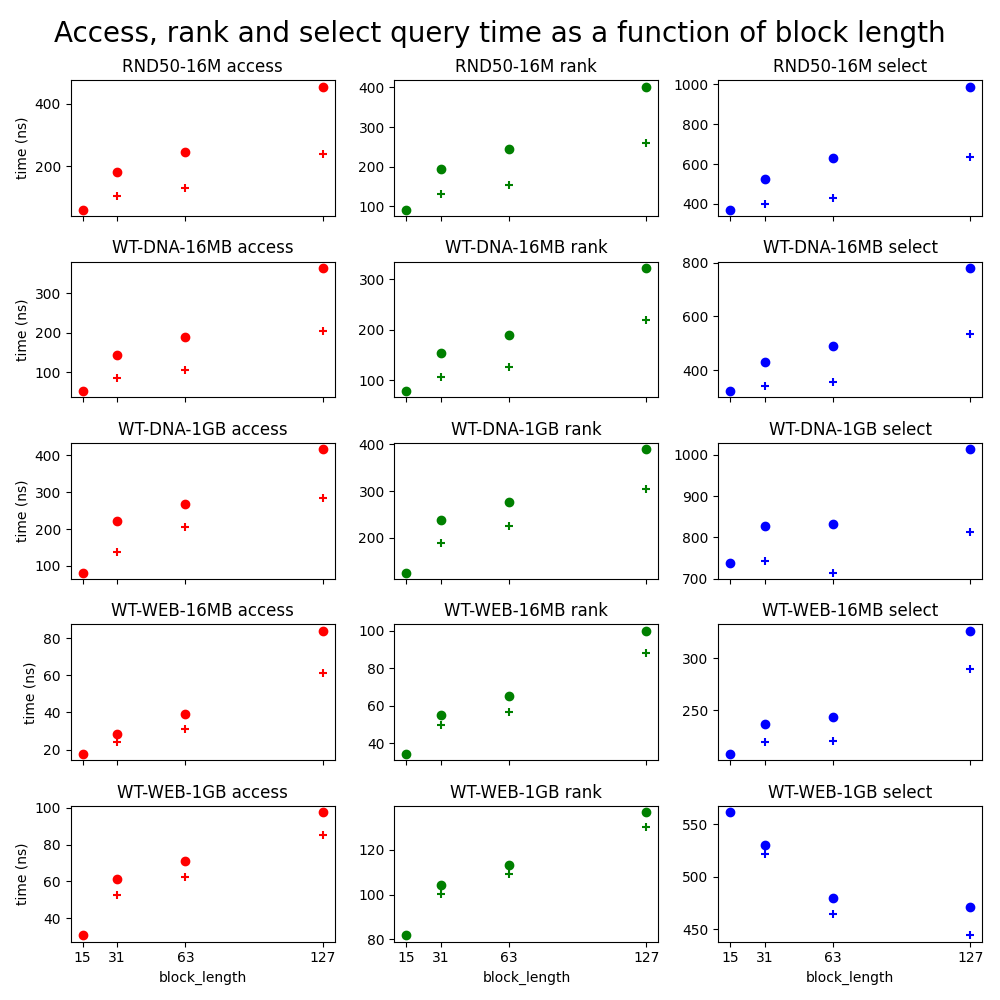
\includegraphics[width=\textwidth, height=0.7\textheight]{images/benchmark_sdsl_new_method}
	}
	\caption[TODO]{\texttt{SDSL} benchmark to measure the bit vector performance and its dependence
	on the block size. Our implementations are marked using cross.
	}
	\label{obr:benchmark_sdsl_new_method}
\end{figure}
There are several interesting things to observe in these results. We can see that our new implementation
beats older implementations on almost all block sizes and all types of data. We can observe that the
results are more clear on random data and DNA sequence. On web data however, the difference is less
noticable. We attribute this behaviour to the fact, that was observed by \cite{gog2014optimized},
creators of this dataset. They observed that the number of uniform blocks (full of either zeroes or ones)
is much bigger in \texttt{WT-WEB} data than in \texttt{WT-DNA}. For block size 63, they observed ratio of
uniform blocks in \texttt{WT-WEB-1GB} to be 84\% compared to 28\% in \texttt{WT-DNA}. As the uniform
blocks are decoded trivially in both implementations, this makes less opportunities for our implementation
to save time.

\paragraph{Bit vector in FM-index}

We further benchmarked our bit vector implementation as a part of Huffman shaped wavelet tree
used inside of the FM-index. Implementation of FM-index in \texttt{SDSL}, as most of other
implementations of FM-index, provides 3 basic methods:

\begin{itemize}
	\item $\countOp(P)$ returns the number of occurrences of $P$ in text $T$
	\item $\locateOp(P)$ returns all positions of pattern $P$ in text $T$
	\item $\extractOp(i, j)$ returns the subsequence $T[i..j]$
\end{itemize}

The reason that the $\extractOp$ method is useful and non-trivial is that FM-index
does not store the original sequence $T$ -- at least not in an easily readable form.
As in previous case, these methods are benchmarked on samples like English texts, \texttt{XML}
data from \texttt{DBLP} as well as on source codes, DNA and protein sequences.
Alongside our new encoding methods and their original counterparts, we once again added
to the benchmark the 15 bit version of bit vector decoded by table. On top of that, we
also added a classic uncompressed bit vector to put into the perspective space savings that
are made by RRR. We present here just a selected subset of the results obtained. We either
choose samples where our implementation beat the original implementation by a wide margin
or others where our implementation was not running that good. All other graphs can be found
in AppendixTODO.

To benchmark operation $\countOp$, the index over the text is built. Then, random patterns of
various lengths are extracted from the text and subsequently used for benchmarking. Code
that generates these patterns in \texttt{SDSL} is a slight modification of a version provided
by \texttt{Pizza\&Chili}.

\begin{figure}
	\centerline{
		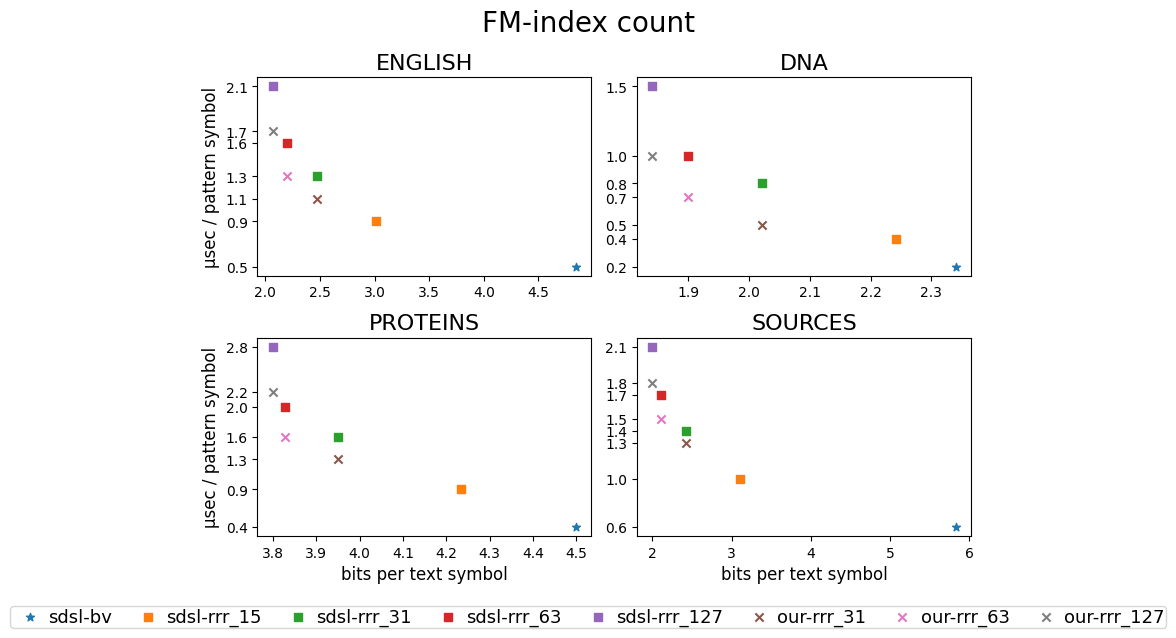
\includegraphics[width=\textwidth, height=0.7\textheight]{images/vysledky_sdsl_count}
	}
	\caption[TODO]{TODO: Zatial iba placeholder obrazok.
	}
	\label{obr:benchmark_sdsl_count}
\end{figure}

For benchmarking of operation $\extractOp$, \texttt{SDSL} uses a methodology proposed by
\cite{ferragina2009compressed} (Section 5.4). This basically consists of extracting numerous
substrings of length 512 starting at random positions in text. There is additional parameter
that is explored in this benchmark - sampling rate of suffix array and inverse suffix array.
This is basically a parameter that can be used to balance the speed of FM-index and its memory
usage. Options for this sampling ratio are the powers of 2 from 4 up to 256. 

\begin{figure}
	\centerline{
		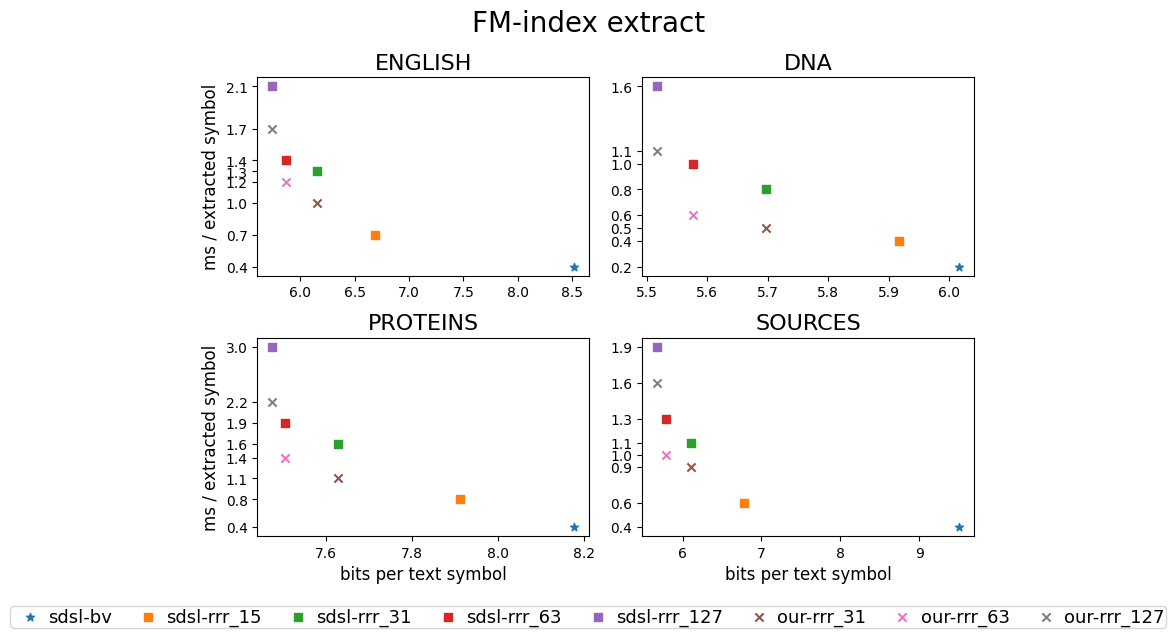
\includegraphics[width=\textwidth, height=0.7\textheight]{images/vysledky_sdsl_extract}
	}
	\caption[TODO]{TODO: Zatial iba placeholder obrazok.
	}
	\label{obr:benchmark_sdsl_extract}
\end{figure}

Benchmarking of operation $\locateOp$ again uses a methodology proposed by \cite{ferragina2009compressed} 
(Section 5.3). This consists of at first locating random patterns of length 5 in the text such
that 2 to 3 millions of occurences are found in the text.

\begin{figure}
	\centerline{
		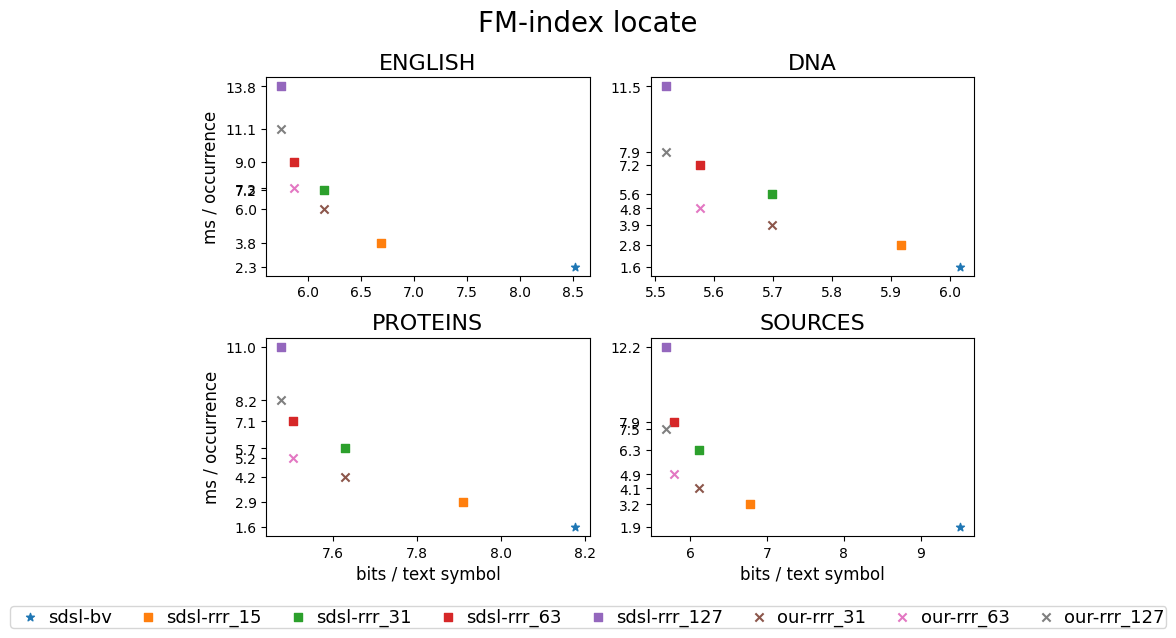
\includegraphics[width=\textwidth, height=0.7\textheight]{images/vysledky_sdsl_locate}
	}
	\caption[TODO]{TODO: Zatial iba placeholder obrazok.
	}
	\label{obr:benchmark_sdsl_locate}
\end{figure}

\paragraph{Correctness}

We wanted to make sure that our implementation is not only as fast possible but also correct. We
used mainly two types of tests for this purpose. The first are the tests of $\access$, $\rank$
and $\select$ functionality in \texttt{SDSL} that run mainly on smaller bit vectors and also cover
special cases that do not happen often in practice such as bit vector full of zeroes/ones. The
second type of tests used was the benchmark running on wavelet tree representation of real data.
Alongside the individual timings, this benchmark produces also as checksum the sum of all the
results of the $\access$, $\rank$ and $\select$ operations.

\section{Hybrid encoding}

\subsection{Implementation}

Implementing hybrid encoding required changes to more than encoding and decoding
subroutines. The first necessary change is addition of hybrid cutoff parameter
to the \texttt{rrr\_vector} class and reimplementation of function \texttt{space\_for\_bt(c)}
that is used in \texttt{SDSL} to get the number of bits that are needed to store offset
of block with class $c$. The second change, more impactful on a runtime
of \texttt{rrr\_vector}, relates to the way how we work with superblocks. When
computing $\rank$ of a bit in particular block, we can still binary search for
the superblock where the $i$-th one is located. To linearly search for a result
inside of the superblock, we need only information from the array of classes $C$.
This is because this array stores the number of ones in the blocks and we can linearly
search for the answer using successive entries of $C$. When we overrun the block, where
the result is located, we go back and find finally answer to $\rank$ inside of a
single block. To locate the beginning of the block, we take the offset of this superblock
in $O$ and add the offset of this block inside of the superblock. The offset from the
beginning of superblock can be counted along with the linear search for $\rank$ result.
With cutoff in place, however, we are not able to linearly scan through the superblock
only using information contained in $C$. This is because now, for some classes, $C$ does
not store the number of ones in the block. Thus when we are linearly searching for the result
of $\rank$ query along the block, we need to also from time to time count number of ones
for some block in $O$. This creates some additional memory accesses that may slow down the
hybrid implementation.

\lstset{language=C++,caption={Rank query, SDSL implementation (pseudo-code)},label=code:binary}
\begin{lstlisting}
int rank(int i)
{
	int block_idx = i/BLOCK_SIZE;
	int superblock_index = block_idx/BLOCKS_PER_SUPERBLOCK;
	int offset = P[superblock_idx];
	int rank  = R[superblock_idx]; // precomputed rank for superblock
	for (int j = superblock_idx*BLOCKS_PER_SUPERBLOCK; j < block_idx; ++j) {
		uint16_t r = C[j];
		rank  += r;
		offset += rrr_helper::space_for_class(r);
	}
	uint16_t off = i % BLOCK_SIZE;
	if (!off) {
		return rank;
	}
	uint16_t c = C[block_idx];

	uint16_t block_length = rrr_helper::space_for_class(c);
	uint32_t o = rrr_helper::get_blocks_offset(O, offset, block_length);
	uint16_t popcnt  = __popcount(rrr_helper::nr_to_bin(c, o) << (32-off));
	return rank + popcnt;
}
\end{lstlisting}

\lstset{language=C++,caption={Rank query, hybrid implementation (pseudo-code)},label=code:binary}
\begin{lstlisting}
int rank(int i)
{
	int block_idx = i/BLOCK_SIZE;
	int superblock_index = block_idx/BLOCKS_PER_SUPERBLOCK;
	int offset = P[superblock_idx];
	int rank  = R[superblock_idx]; // precomputed rank for superblock
	for (int j = superblock_idx*BLOCKS_PER_SUPERBLOCK; j < block_idx; ++j) {
		uint16_t r = C[j];
		if (r >= c_k) {
			uint32_t o = rrr_helper::get_blocks_offset(O, offset, BLOCK_SIZE);
			rank += __popcount(btnr);
		}
		else {
			rank  += r;
		}
		offset += rrr_helper::space_for_class(r);
	}
	uint16_t off = i % BLOCK_SIZE;
	if (!off) {
		return rank;
	}
	uint16_t c = C[block_idx];

	uint16_t block_length = rrr_helper::space_for_class(c);
	uint32_t o = rrr_helper::get_blocks_offset(O, offset, block_length);
	uint16_t popcnt  = __popcount(rrr_helper::nr_to_bin(c, o) << (32-off));
	return rank + popcnt;
}
\end{lstlisting}

\subsection{Experimental results}

\begin{figure}
	\centerline{
		\includegraphics[width=\textwidth, height=0.4\textheight]{images/benchmark_sdsl_hybrid}
	}
	\caption[TODO]{\texttt{SDSL} benchmark to measure the bit vector performance and its dependence
	on the block size. Our implementations are marked using cross.
	}
	\label{obr:benchmark_sdsl_hybrid}
\end{figure}